\begin{frame}{Traitement du signal audio-numérique}
\begin{block}{Besoins et problématiques associées}
\structure{Transmission}: Codage \\
\structure{Indexation}: Recherche d'Information (IR) \\
\structure{Création}: Synthèse sonore
\end{block}
\begin{block}{Domaines d'application}
\begin{itemize}
\item Musique
\item Sons environnementaux
\end{itemize}
\end{block}
\end{frame}


\begin{frame}{Besoins de compacité}
\begin{block}{Verrou}
\begin{itemize}
\item une seconde de son : $$ x \in \mathbb{R}^{44100}$$
\item besoin d'une représentation plus \alert{compacte}
\end{itemize}
\end{block}
\begin{block}{Types de compacité}
\structure{Codage}: compacité signal \\ % ($ y \in \mathbb{R}^{5000}$) \\
\structure{Recherche d'information}: compacité sémantique \\ %  ($ y \in \mathbb{N}^{100}$) \\
\structure{Synthèse}: compacité \alert{\og} \structure{signalo-sémantique} \alert{\fg} \\ %  ($ y \in \mathbb{R}^{100}$)
\end{block}
\end{frame}

\begin{frame}{Codage compressif par transformée}
$$y = C(x) | \tilde{x} = C^{-1}(y), P_e(x) \simeq P_e(\tilde{x})$$
\begin{itemize}
\item $C$ : Quantification adaptative d'un équivalent de la Transformée de Fourier à Court Terme (TFCT)
\item $P_e$ : Modélisation de la sensibilité aux déformations de la membrane basilaire\footfullcitenomarkleft{zwicker2013psychoacoustics}
\end{itemize}
\end{frame}

\begin{frame}{Transformée de Fourier à Court Terme (TFCT)}
$$ f[m, t] = \sum_{n = - \infty}^{\infty} x[n] w[n-t] \mathrm{e}^{\frac{-2 \mathrm{j}  \pi m n}{N}} $$

\begin{description}
\item[$x$]: signal temporel
\item[$f$]: composantes fréquentielles (paniers, bins, ...)
\item[$w$]: fenêtre
\end{description}
\footfullcitenomarkleft{lostanlen2019fourier}
\end{frame}

\begin{frame}{Spectrogramme : $|f[m, t]|$}
\begin{center}
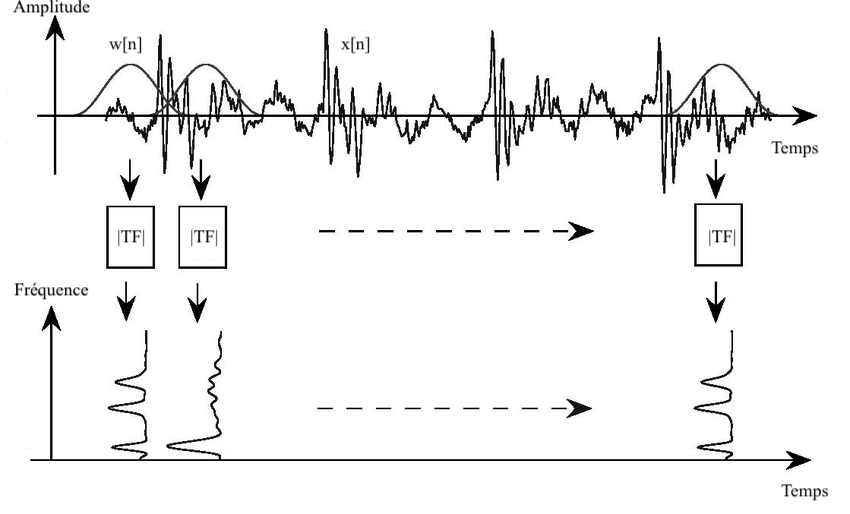
\includegraphics[width=.8\columnwidth]{figures/tfct} \\
\end{center}
\end{frame}

\begin{frame}{Spectrogramme}
\begin{center}
\only<1>{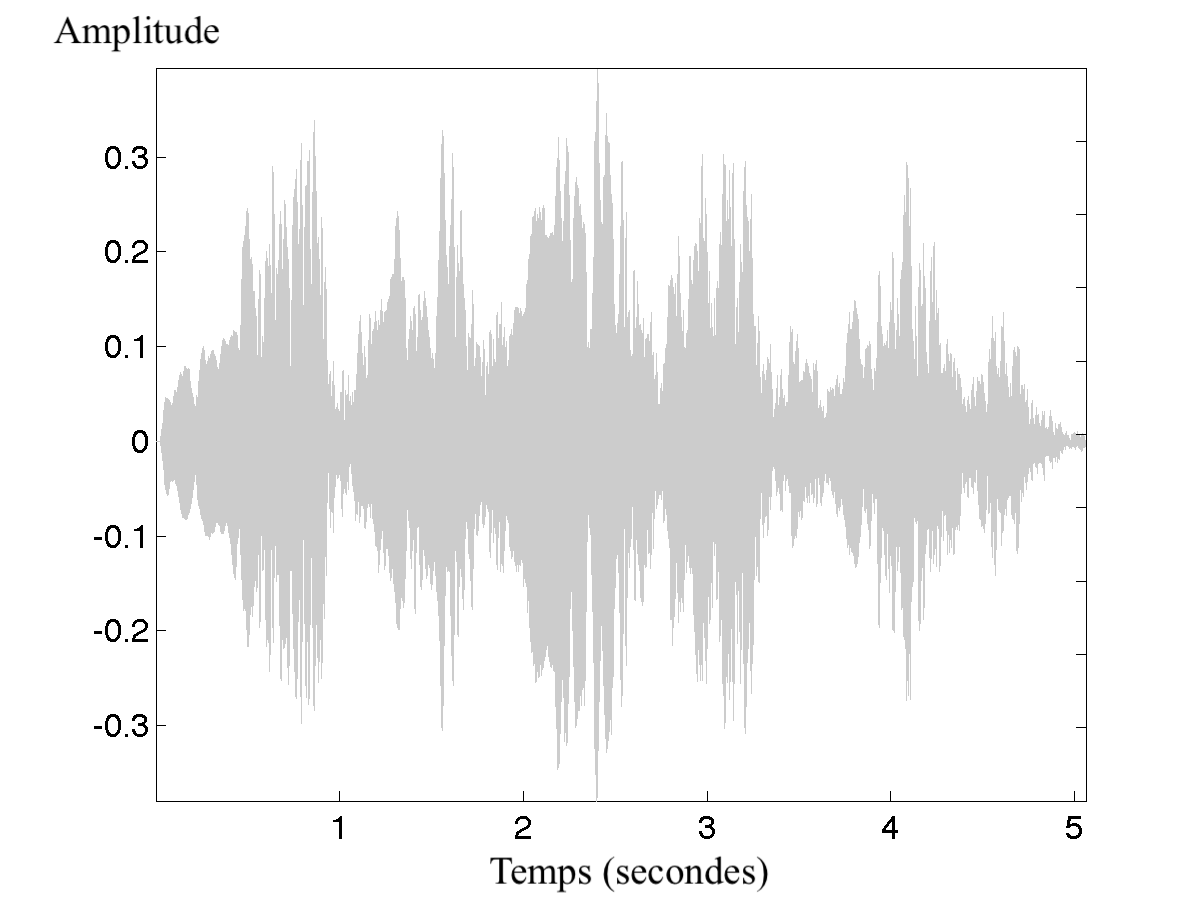
\includegraphics[width=.8\columnwidth]{figures/soloTime}}
\only<2>{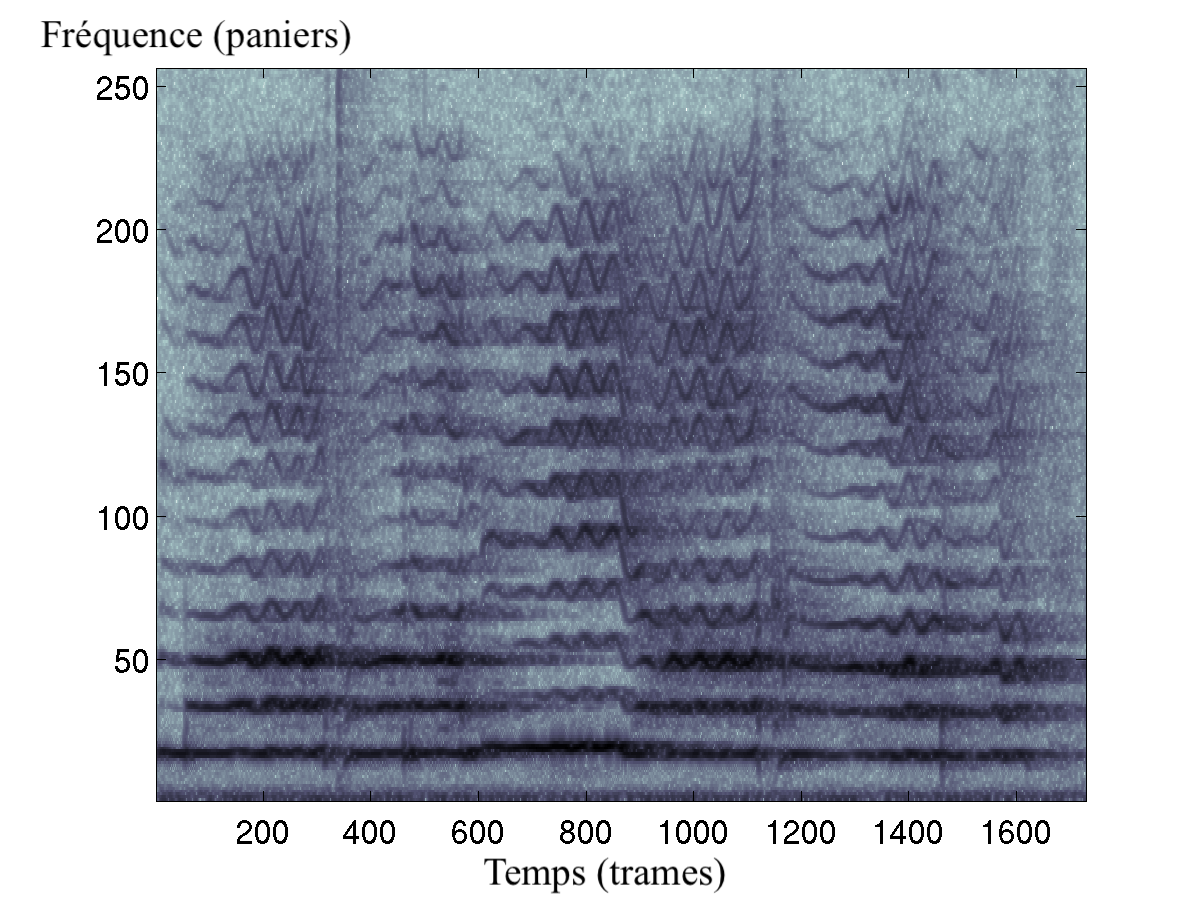
\includegraphics[width=1.1\columnwidth]{figures/soloSpec}}

\includesound{sounds/solo.mp3}
\end{center}
\end{frame}

\begin{frame}{Typologie des évènements sonores}
  \begin{tabular}{l|cc}
    & \multicolumn{2}{c}{structure} \\
  \structure{sons}  & horizontale & verticale \\
    \hline
    \structure{de parole} & sons voisés & sons plosifs  \\
    & <a>, <o> &  <pe>, <qe> \\
    \structure{d'animaux} & chants & clics  \\
    \structure{musicaux} & chant lyrique & percussions \\
    \structure{mécaniques} & ventilation & marteau piqueur \\
    \structure{environnementaux} & vent & gouttes de pluie \\
  \end{tabular}
\end{frame}

\begin{frame}{Compromis temps/fréquence}
	$\hookrightarrow{}$ mitiger cette contrainte imposée par l'approche court-terme par l'utilisation d'\alert{\textit{a priori}} sur les sources d'intérêt.
\end{frame}
